\section{Algorithms}
In this chapter, we will present all used algorithms and models for both classification tasks. The presented examples in this chapter are all using BERT for validity classification. All steps work analogously for RoBERTa and stance detection. The only difference is the input for the LMs since the data for stance detection looks a little bit different.

\subsection{Baseline}
To compare the performance of our models, we use simple BERT and RoBERTa classifier \cite{bert, roberta} as baseline. We use the training procedure and model from huggingface \cite{berttraining} with the standard parameters proposed in the original BERT paper \cite{bert}. More details can be found in the implementation chapter.

\subsection{Approach}

This section is about describing all the necessary steps for our approach and explaining why we thought these steps are sensible. The approach consists of the following steps, as shown for BERT in figure \ref{fig:model-architecture1}:

\begin{enumerate}
	\item Generate embeddings for each data point based on probabilities for linking words.
	\item Concatenate these embeddings with LM embeddings.
	\item Classify the combined embeddings.
\end{enumerate}

\begin{figure}[h]
  \centering
  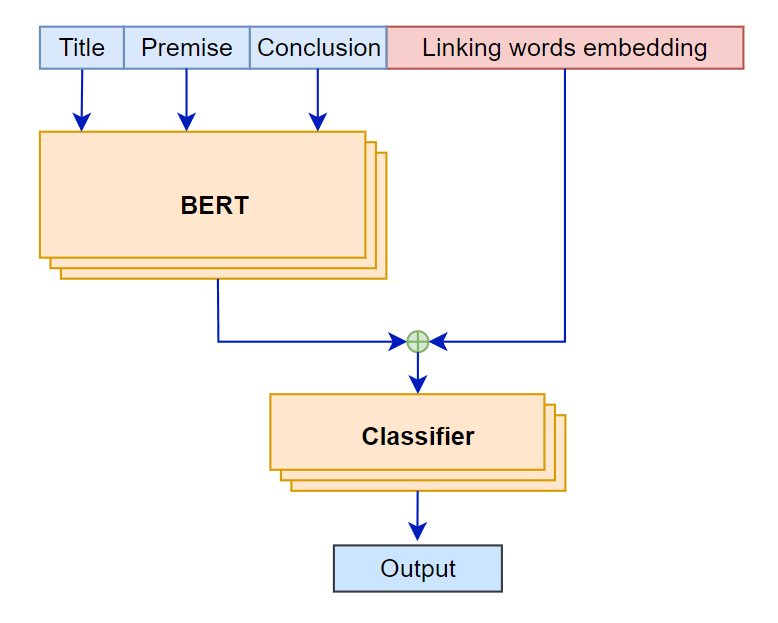
\includegraphics[scale=0.6]{fig/model_diag1.png}
  \caption{Model Architecture for validity classification with BERT: BERT transforms the text to an embedding. This is concatenated with the linking words embedding and then classified.}%
  \label{fig:model-architecture1}
\end{figure}

The main idea of our algorithm as described in the introduction, comes from the idea of using linking words to connect sentences in a meaningful way. Often times in natural language, conclusions or arguments are indicated using linking words like \dq therefore\dq or \dq thus\dq. We want to use this fact to improve the performance of our baseline model by combining embeddings generated by LMs with custom embeddings depending on probabilities of these linking words being at the start of the conclusion/argument. In the next section, we will discuss exactly how these custom embeddings are created.

\subsubsection{Embeddings based on linking word probabilities} \label{sec:linkingembeddings}
To generate our custom embeddings, we will use LMs for masked language modeling. We start by finetuning a LM for masked language modeling \cite{bertmask} on either the validity or the stance dataset. Optionally we use the ChatGPT dataset before. For all three datasets, we just take one data point as one input sequence without [SEP] tokens in between the sentences, regardless of the number of sentences. After training, we add a [MASK] token to the start of every conclusion/argument (directly after the <\_c> marker). This extended data is then used to let the LM predict words for the [MASK] token. The LM yields a list of all the words in the vocabulary and their corresponding probabilities to be at the position of that [MASK] token. Now we define a set of linking words $\mathcal{L}$ and extract the probabilities for each linking word of $\mathcal{L}$ from the list of probabilities from the LM. This gives us a vector $E$ of probabilities with length $|\mathcal{L}|$ which is the final embedding for one datapoint. We will repeat this for every data point. \\

When looking at this embedding however, we can see one problem. The probabilities tend to be very low and therefore the differences between probabilities are very low. One possible explanation could be that the data on which the LM was originally trained on, does not contain a lot of our chosen linking words and hence gives them a relatively low probability compared to more common words which would also fit in this position. One way to increase these values is to compare them to another value and use the relative difference as new value. We decided to do that in the following way: \\
Given a word vector embedding $E$, we build a matrix $M_E$ by applying the outer product between $E$ and $\frac{1}{E}$: $M_E = E \otimes \frac{1}{E} = E \cdot (\frac{1}{E})^T$.
Afterwards, we remove the diagonal entries of this matrix since these are all $1$ to get $M_E'$ and transform this matrix row wise into a vector: $E_{matrix} = vec(M_E')$ (see figure \ref{fig:transform1}). This new embedding has length $|\mathcal{L}| \cdot (|\mathcal{L}|-1)$.

\begin{figure}[h]
	\centering
	$$ M_E = \begin{pmatrix}
		e_1\\
        e_2\\
        \vdots\\
        e_{|\mathcal{L}|}
     \end{pmatrix}
     \cdot
     \begin{pmatrix}
     	\frac{1}{e_1} & \frac{1}{e_2} & \cdots & \frac{1}{e_{|\mathcal{L}|}}
     \end{pmatrix} = 
	 \begin{pmatrix}
		\frac{e_1}{e_1} & \frac{e_1}{e_2} & \cdots & \frac{e_1}{e_{|\mathcal{L}|}}\\
        \frac{e_2}{e_1} & \frac{e_2}{e_2} & \cdots & \frac{e_2}{e_{|\mathcal{L}|}}\\
        \vdots & \vdots & \ddots & \vdots\\
        \frac{e_{|\mathcal{L}|}}{e_1} & \frac{e_{|\mathcal{L}|}}{e_2} & \cdots & \frac{e_{|\mathcal{L}|}}{e_{|\mathcal{L}|}}
     \end{pmatrix}     
     $$
     
     $$
	 M_E' =   
	 \begin{pmatrix}
		\frac{e_1}{e_2} & \frac{e_1}{e_3} & \cdots & \frac{e_1}{e_{|\mathcal{L}|}}\\
        \frac{e_2}{e_1} & \frac{e_2}{e_3} & \cdots & \frac{e_2}{e_{|\mathcal{L}|}}\\
        \vdots & \vdots & \ddots & \vdots\\
        \frac{e_{|\mathcal{L}|}}{e_1} & \frac{e_{|\mathcal{L}|}}{e_2} & \cdots & \frac{e_{|\mathcal{L}|}}{e_{|\mathcal{L}|-1}}
     \end{pmatrix}  
     $$
     
     $$
     E_{matrix} = vec(M_E') = 
     \begin{pmatrix}
     	\frac{e_1}{e_2}  \frac{e_1}{e_3}  \cdots  \frac{e_1}{e_{|\mathcal{L}|}}  \frac{e_2}{e_1}  \frac{e_2}{e_3}  \cdots \frac{e_2}{e_{|\mathcal{L}|}}  \cdots  \frac{e_{|\mathcal{L}|}}{e_1} \frac{e_{|\mathcal{L}|}}{e_2}  \cdots  \frac{e_{|\mathcal{L}|}}{e_{|\mathcal{L}|-1}}
     \end{pmatrix}^T
     $$
     
	\caption{Transformation from $E$ to $E_{matrix}$}%
	\label{fig:transform1}
\end{figure}

In the following chapters, we will always use $E$ as embedding to describe the other steps. They work analogously for $E_{matrix}$. \\

We also chose to apply another method to calculate the embedding for validity classification only. Since in the validity classification dataset, most of the premises consist of more than one sentence (in the stance detection dataset most statements are exactly one sentence), we change masking in the following way: \\
\begin{enumerate}
	\item For each datapoint, split the sentences of the premise.
	\item Append "<\_c> [MASK] \textit{conclusion}" at each sentence.
	\item Calculate probabilities for linking words at the [MASK] token position as before for each sentence conclusion pair.
	\item Take the maximum probability for all linking words along all the sentences to generate a new embedding for this datapoint.
\end{enumerate}

\subsubsection{BERT and RoBERTa embeddings} \label{sec:bertembeddings}
As described in chapter 2, BERT outputs a vector representation for each token in the sequence, including special tokens. To generate embeddings for the entire sequence, we have to somehow transform these vectors into one. The following approach works for BERT aswell as for RoBERTa.\\
Given an input sequence of length $l$, including all special tokens, BERT produces an output representation of shape ($l$, $H$) where $H$ is the hidden dimension of BERT (in our case always $768$). We will use two different ways to generate an embedding of shape ($1$, $H$) which we can then use for classification. The first way is the standard way explained in chapter 2, proposed by Devlin et. al. \cite{bert}. It assumes that the first token in the sequence, namely the [CLS] token, can be used as an aggregate representation of the entire sequence an hence be a suitable embedding for it. The other way is taking the average of all the token vectors along the first dimension. Both ways yield the desired embedding vector of shape ($1$, $H$).

\subsubsection{Classifier}
We are using two different classifiers. The first one is a simple neural net. We use the same architecture as the one that is used in BertForSequenceClassification from the transformer package \cite{bertimpl}. It consists of one dropout layer and one linear layer, followed by a softmax layer and the loss function, as shown in figure \ref{fig:nn1}. In the case of using the concatenated embeddings, the linear layer transforms the input matrix from shape $(D, \, |E| + H)$ to shape ($D$, $2$) where $D$ is the number of data points in the dataset. 

\begin{figure}[h]
  \centering
  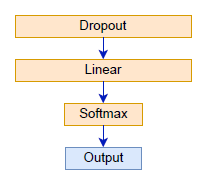
\includegraphics[scale=1]{fig/nn_1.png}
  \caption{Neural network classifier.}%
  \label{fig:nn1}
\end{figure}

For the second classifier, we will use a gradient-boosted tree, precisely LightGBM \cite{lgbm}.

\subsubsection{Feature selection}
Before passing the embedding vectors to the classifier, we apply feature selection to improve the performance of our model, by discarding features with low importance. This importance is calculated by the built-in method of LightGBM \cite{lgbmimportance}. We use different metrics to decide below which importance features are discarded, e.g. discarding all features whose importance is below the mean importance. The best working metric for us is discarding all features whose importance is $\frac{\text{average importance}}{4}$. This will be discussed in more detail in the implementation chapter.

\subsubsection{Summary}
Combining all steps, gives us the model shown in figure \ref{fig:model-architecture_full}. We will evaluate all the introduced techniques in different configurations. All the exact configurations will be explained in the evaluation chapter.

\begin{figure}[h]
  \centering
  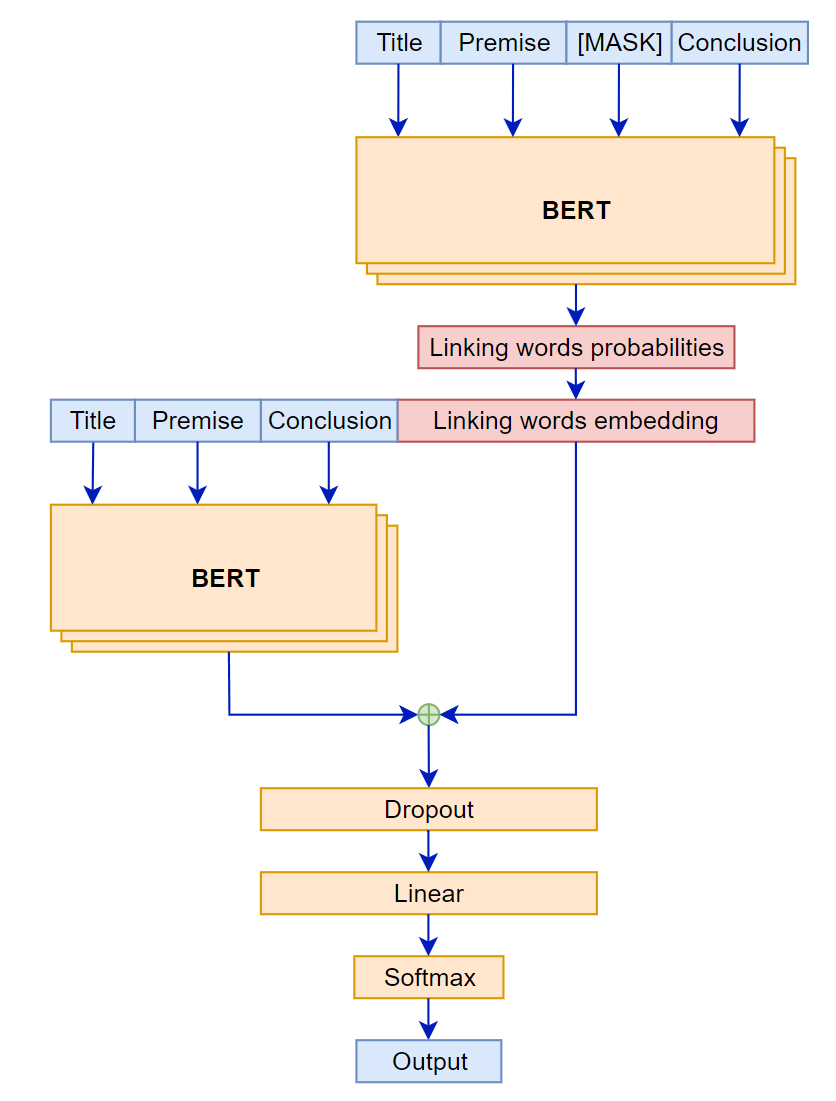
\includegraphics[scale=0.6]{fig/model_complete.png}
  \caption{Complete Model Architecture for validity classification with BERT.}%
  \label{fig:model-architecture_full}
\end{figure}









